
%%%%%%%%%%%%%%%%%%%%%%%%%%%%%%%%%%%%%%%%%%%%%%%%%%%%%%%%%%%%%%%%%%%%%%%%
%Para las ecuaciones siempre es Ec.(n).
%Para las figuras siempre es Fig.n, incluso en el caption de la figura. Tambien las Tablas
%Para las referencias es [n]
%%%%%%%%%%%%%%%%%%%%%%%%%%%%%%%%%%%%%%%%%%%%%%%%%%%%%%%%%%%%%%%%%%%%%%%%

\documentclass[
reprint,
%notitlepage,
%superscriptaddress,
%groupedaddress,
%unsortedaddress,
%runinaddress,
%frontmatterverbose, 
%preprint,
%showpacs,preprintnumbers,
%nofootinbib,
%nobibnotes,
%bibnotes,
%11 pt,
amsmath,
amssymb,
aps,
pra,
%prb,
%rmp,
%tightenlines %esto hizo el milagro de sacar los espacios en blancos estocásticos (?)
 %prstab,
%prstper,
%floatfix,\textbf{}
]{revtex4-1} %Instalar primero para usarlo. Paquete malo.

%\documentclass[onecolumn, aps, amsmath,amssymb ]{article}
\usepackage{lipsum}  
\usepackage{graphicx}% Include figure files
\usepackage{subfig}
\usepackage{braket}
\usepackage{comment} %comment large chunks of text
\usepackage{dcolumn}% Align table columns on decimal point
\usepackage{bm}% bold math
%\usepackage{hyperref}% add hypertext capabilities
\usepackage[mathlines]{lineno}% Enable numbering of text and display math
%\linenumbers\relax % Commence numbering lines
\usepackage{mathtools} %% Para el supraíndice

\usepackage[nice]{nicefrac}

%%%%%%%El Señor Español%%%%%%%%%%%%%%%%%%%%%%%%%%%
\usepackage[utf8]{inputenc} %acento
\usepackage[
spanish, %El lenguaje.
es-tabla, %La tabla y no cuadro.
activeacute, %El acento.
es-nodecimaldot %Punto y no coma con separador de números
]{babel}
\usepackage{microtype} %para hacerlo más bonito :33 como vos (?) 
%%%%%%%%%%%%%%%%%%%%%%%%%%%%%%%%%%%%%%%%%%%%%%%%%%%
%%%%%%%%% Para que las imágenes se queden dónde las quiero (?
\usepackage{float}
%%%%%%%%%%

%%%%%%%%Cambia a Fig de Figure%%%%%%%%%%
\makeatletter
\renewcommand{\fnum@figure}{Fig. \thefigure} 
\makeatother
%%%%%%%%%%%%%%%%%%%%%%%%%%%%%%%%%%%%%%%%
\raggedbottom

\usepackage{hyperref}
\begin{document}
%%%%%%%%%%%%%%%%%%%%%%%%%%%%%%%%%%Título%%%%%%%%%%%%%%%%%%%%%%%%%%%%%%%%%%%%%%
%%%%%%%%%%%%%%%%%%%%%%%%%%%%%%%%%%%%%%%%%%%%%%%%%%%%%%%%%%%%%%%%%%%%%%%%%%%%%%

\title{Práctica 3: Estadística de trenes de spikes }
\author{Evelyn~G.~Coronel}

\affiliation{
Redes~Neuronales - Instituto~Balseiro\\}

\date[]{\lowercase{\today}} %%lw para lw, [] sin date

\begin{abstract}
Soluciones a los ejercicios de la práctica 3 de la materia de Redes Neuronales. En esta práctica se estudia la estadística de los resultados obtenidos para un experimento. En mismo se excita una neurona con un estimulo oscilatorio.
\end{abstract} 
\maketitle
%%%%%%%%%%%%%%%%%%%%%%%%%%%%%%%%%%%%%%%%%%%%%%%%%%%%%%%%%%%%%%%%%%%%%%%%%%%%%%%%%%%

\section*{Estimulo}

\begin{figure}[H]
	\centering
	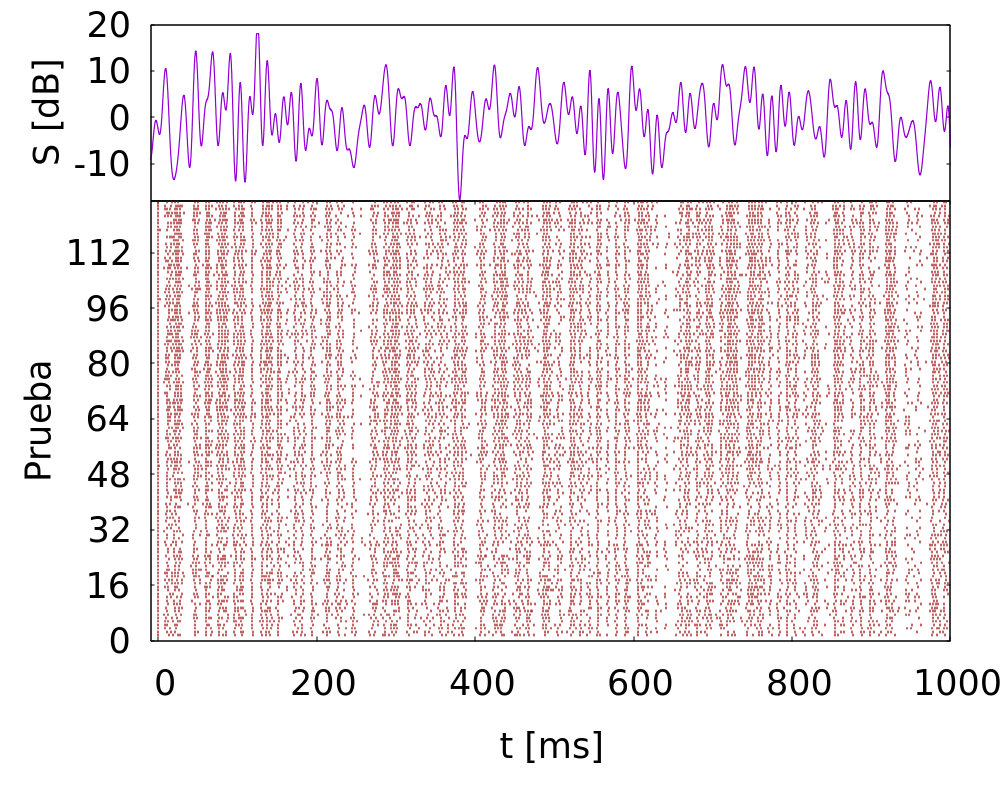
\includegraphics[width=0.5\textwidth]{../Graficos/stimulus.png}
	\caption{La intensidad del estimulo en función de tiempo. La misma representa un sonido que estimula a un insecto.}
\end{figure}


La varianza del estimulo es de $\sigma^2_{s}= 31.649\,$dB$^2$
\section*{Distribución de intervalos \texorpdfstring{$P(\tau)$}{}}

\begin{figure}[H]
	\centering
	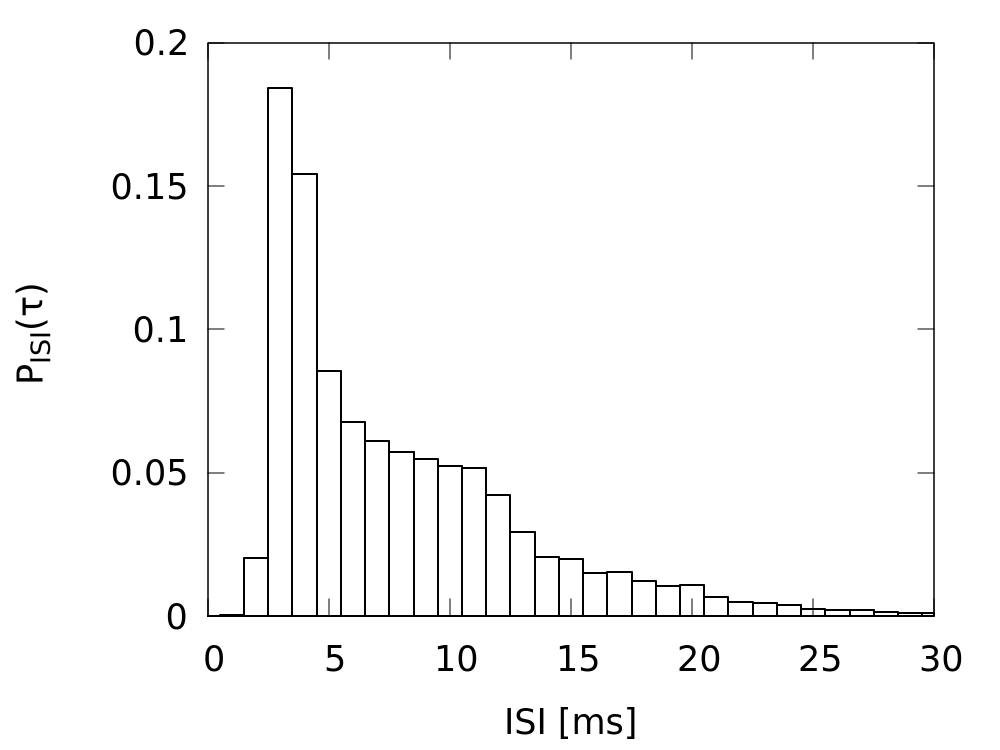
\includegraphics[width=0.5\textwidth]{../Graficos/p_isi.png}
	\caption{Distribución de probabilidad de los valores del ISI}
	\end{figure}


La distribución tiene una media de $\langle ISI \rangle = 84.68\,$ms y un varianza de $\sigma^2_{ISI}=3111.96\,$ms$^2$.
El factor $CV=0.659$


\section*{Distribución de número de spikes \texorpdfstring{$P(N)$}{}}

\begin{figure}[H]
	\centering
	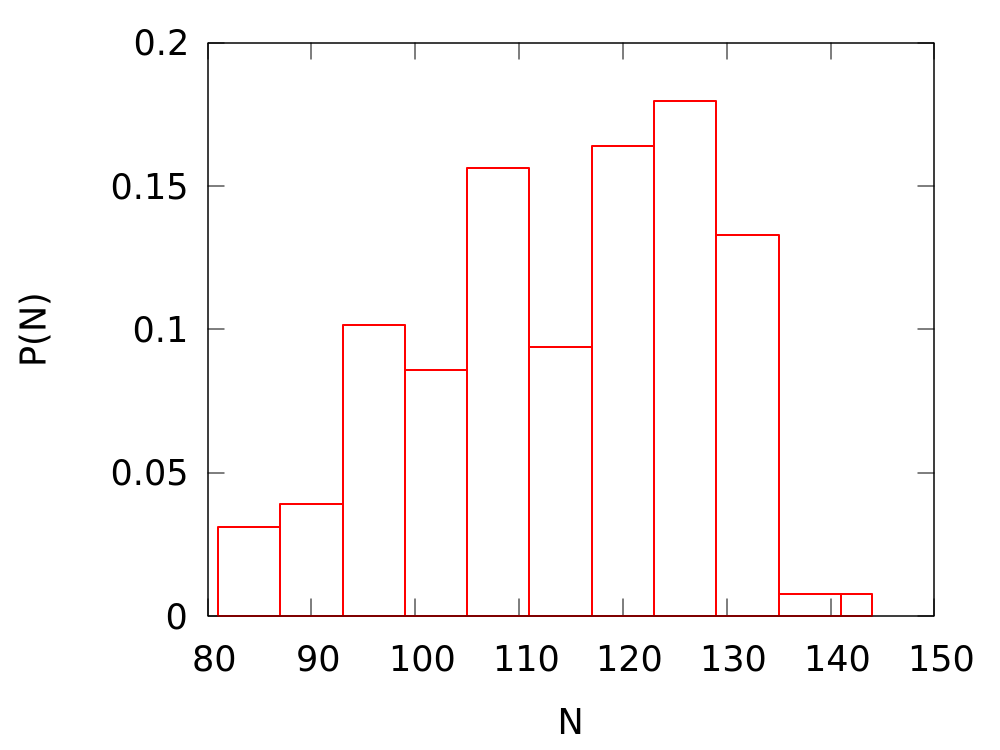
\includegraphics[width=0.5\textwidth]{../Graficos/p_N.png}
	\caption{Distribución de probabilidad de la cantidad de spikes en cada realización del experimento.}
\end{figure}


La distribución tiene una media de $\langle N \rangle = 117.01$ y un varianza de $\sigma^2_{N}=183.195$.
El factor de Fano $F=1.567$


\section*{Histograma de la tasa de disparo \texorpdfstring{$r(t)$}{}}


\begin{figure}[H]
	\centering
	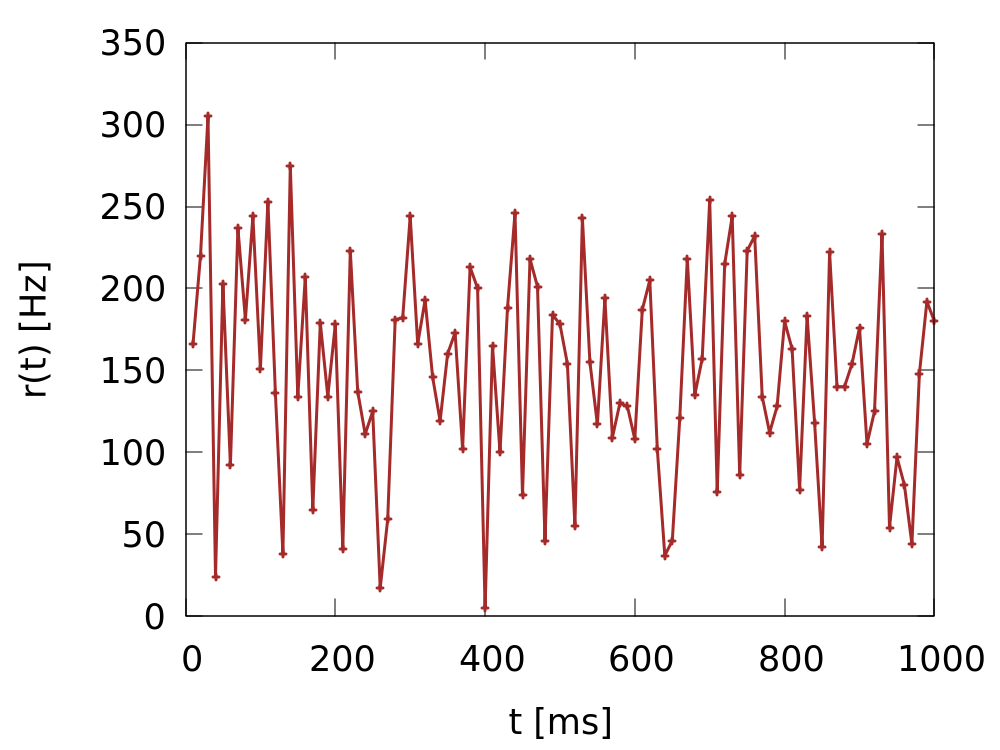
\includegraphics[width=0.5\textwidth]{../Graficos/r_t.png}
	\caption{Tasa de disparo subyacente}
\end{figure}

\section*{Filtro asociado a la neuronas \texorpdfstring{$D(\tau)$}{}}


Considerando que la señal es ruido blanco, es decir que $Q_{s,s}(\tau, \tau')= \sum_{spikes} \sigma^2_s \delta(\tau-\tau')$, se obtiene que el filtro asociado es 
\begin{align}
    D(\tau) &= \frac{Q_{r,s}(-\tau)}{\sigma^2}, \\
    \text{con } Q_{r,s}(-\tau) &= \sum_{spikes} S(t_{spike} - \tau)
\end{align}
donde $S(t)$ es el valor del estimulo al tiempo $t$


\end{document}

